Trong bài tập này, ta sẽ gọi các ký hiệu như sau 

\begin{description}
    \item[R] Bán kính của hộp đen quang học
   \item [$\theta$] Góc quay của hộp đen quang học
   \item [$\alpha$] Góc laser thu được
   \item [$h$] Đường cao kẻ từ O xuống một cạnh
   \item [$\beta$] Góc tới so với gương
\end{description}


\begin{enumerate}
\item 
Khi nhìn vào đồ thị đề bài thì ta sẽ rút ra được được một số điều như sau:
\begin{enumerate} 
    \item Có 4 điểm bị gián đoạn trong khoảng từ $0^\circ$ đến $360^\circ$. Như vậy sẽ có hình dạng của vật kính là một hình tam giác (vì điểm gián đoạn ở điểm $\theta=0$ và $\theta=360^\circ$ trùng nhau).
    \item Do cách sự gián đoạn là đều, đối xứng nên hình dạng của vật kính buộc phải là một hình đều.
    \item Điểm gián đoạn có toạ độ trong đồ thị $(\theta;\alpha)$ là $\left(k.120^\circ ; \pm 110^\circ \right)$.
    \item Điểm mà $\alpha=0^\circ$ là lúc mà laser vuông góc với lại một trong các tấm kính, có toạ độ là $\left( (n+1) \cdot 60^\circ ; 0^\circ \right)$.
\end{enumerate}
Từ những nhận định trên, ta có thể khẳng định được là vật kính bên trong hộp đen quang học có dạng là một lăng trụ tam giác đều. Và tại thời điểm ban đầu, tia laser chiếu qua một đỉnh của vật.
\\Xét tại một điểm gián đoạn trong đồ thị, ở đây là ta chọn là $\left(0;110^\circ \right)$. 
\begin{center}
    





\tikzset{every picture/.style={line width=0.75pt}} %set default line width to 0.75pt        

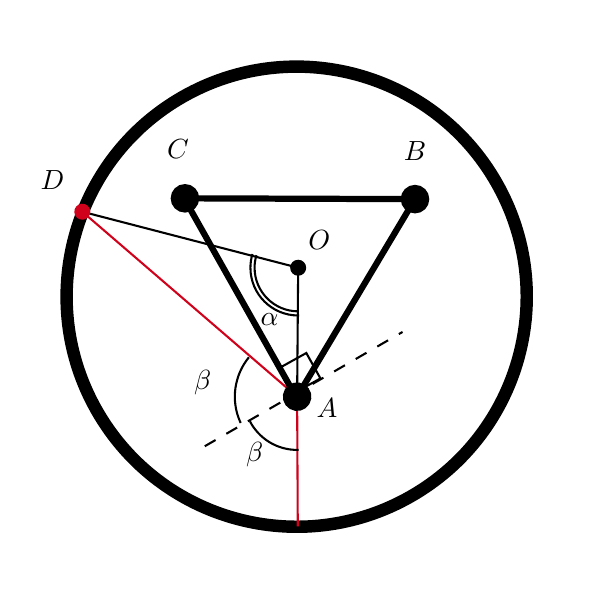
\begin{tikzpicture}[x=0.75pt,y=0.75pt,yscale=-1,xscale=1]
%uncomment if require: \path (0,1136); %set diagram left start at 0, and has height of 1136

%Straight Lines [id:da3728532088409502] 
\draw    (406,567.5) -- (510,594.5) ;
%Shape: Ellipse [id:dp5793362401453883] 
\draw  [line width=4.5]  (564.19,704.71) .. controls (511.02,735.04) and (443.33,716.52) .. (413,663.35) .. controls (382.68,610.18) and (401.19,542.49) .. (454.36,512.17) .. controls (507.53,481.84) and (575.22,500.36) .. (605.55,553.53) .. controls (635.88,606.7) and (617.36,674.38) .. (564.19,704.71) -- cycle ;
%Straight Lines [id:da6194863690570493] 
\draw [color={rgb, 255:red, 208; green, 2; blue, 27 }  ,draw opacity=1 ]   (406,567.5) -- (509.49,656.62) ;
\draw [shift={(406,567.5)}, rotate = 40.73] [color={rgb, 255:red, 208; green, 2; blue, 27 }  ,draw opacity=1 ][fill={rgb, 255:red, 208; green, 2; blue, 27 }  ,fill opacity=1 ][line width=0.75]      (0, 0) circle [x radius= 3.35, y radius= 3.35]   ;
%Straight Lines [id:da21803442459681333] 
\draw [color={rgb, 255:red, 208; green, 2; blue, 27 }  ,draw opacity=1 ]   (509.81,719.12) -- (509.49,656.62) ;
%Straight Lines [id:da4551603999688445] 
\draw [line width=2.25]    (455.45,561.05) -- (566.28,561.44) ;
\draw [shift={(566.28,561.44)}, rotate = 0.2] [color={rgb, 255:red, 0; green, 0; blue, 0 }  ][fill={rgb, 255:red, 0; green, 0; blue, 0 }  ][line width=2.25]      (0, 0) circle [x radius= 5.36, y radius= 5.36]   ;
\draw [shift={(455.45,561.05)}, rotate = 0.2] [color={rgb, 255:red, 0; green, 0; blue, 0 }  ][fill={rgb, 255:red, 0; green, 0; blue, 0 }  ][line width=2.25]      (0, 0) circle [x radius= 5.36, y radius= 5.36]   ;
%Straight Lines [id:da6523806158389662] 
\draw [line width=2.25]    (509.49,656.62) -- (566.28,561.44) ;
\draw [shift={(509.49,656.62)}, rotate = 300.82] [color={rgb, 255:red, 0; green, 0; blue, 0 }  ][fill={rgb, 255:red, 0; green, 0; blue, 0 }  ][line width=2.25]      (0, 0) circle [x radius= 5.36, y radius= 5.36]   ;
%Straight Lines [id:da3237474567258274] 
\draw [line width=2.25]    (509.69,658) -- (455.28,561.44) ;

%Straight Lines [id:da2545714169817601] 
\draw    (509.49,656.62) -- (510,594.5) ;
\draw [shift={(510,594.5)}, rotate = 270.47] [color={rgb, 255:red, 0; green, 0; blue, 0 }  ][fill={rgb, 255:red, 0; green, 0; blue, 0 }  ][line width=0.75]      (0, 0) circle [x radius= 3.35, y radius= 3.35]   ;
\draw [shift={(509.49,656.62)}, rotate = 270.47] [color={rgb, 255:red, 0; green, 0; blue, 0 }  ][fill={rgb, 255:red, 0; green, 0; blue, 0 }  ][line width=0.75]      (0, 0) circle [x radius= 3.35, y radius= 3.35]   ;
%Straight Lines [id:da24286904370485152] 
\draw  [dash pattern={on 4.5pt off 4.5pt}]  (465,680.5) -- (560.28,625.44) ;
%Shape: Arc [id:dp16465728093915843] 
\draw  [draw opacity=0] (510.41,617.5) .. controls (510.27,617.5) and (510.14,617.5) .. (510,617.5) .. controls (497.3,617.5) and (487,607.2) .. (487,594.5) .. controls (487,592.2) and (487.34,589.98) .. (487.96,587.89) -- (510,594.5) -- cycle ; \draw   (510.41,617.5) .. controls (510.27,617.5) and (510.14,617.5) .. (510,617.5) .. controls (497.3,617.5) and (487,607.2) .. (487,594.5) .. controls (487,592.2) and (487.34,589.98) .. (487.96,587.89) ;  
%Shape: Arc [id:dp559379065616912] 
\draw  [draw opacity=0] (482.3,669.29) .. controls (482.23,669.13) and (482.15,668.97) .. (482.08,668.81) .. controls (477.32,658.11) and (479.33,646.12) .. (486.26,637.63) -- (509.49,656.62) -- cycle ; \draw   (482.3,669.29) .. controls (482.23,669.13) and (482.15,668.97) .. (482.08,668.81) .. controls (477.32,658.11) and (479.33,646.12) .. (486.26,637.63) ;  
%Shape: Arc [id:dp9563767479981979] 
\draw  [draw opacity=0] (510.37,615.5) .. controls (510.25,615.5) and (510.12,615.5) .. (510,615.5) .. controls (498.4,615.5) and (489,606.1) .. (489,594.5) .. controls (489,592.4) and (489.31,590.38) .. (489.88,588.46) -- (510,594.5) -- cycle ; \draw   (510.37,615.5) .. controls (510.25,615.5) and (510.12,615.5) .. (510,615.5) .. controls (498.4,615.5) and (489,606.1) .. (489,594.5) .. controls (489,592.4) and (489.31,590.38) .. (489.88,588.46) ;  
%Shape: Arc [id:dp1155030999612674] 
\draw  [draw opacity=0] (510.22,682.25) .. controls (510.07,682.25) and (509.92,682.26) .. (509.77,682.26) .. controls (499.77,682.37) and (491.04,676.73) .. (486.72,668.42) -- (509.49,656.62) -- cycle ; \draw   (510.22,682.25) .. controls (510.07,682.25) and (509.92,682.26) .. (509.77,682.26) .. controls (499.77,682.37) and (491.04,676.73) .. (486.72,668.42) ;  
%Shape: Square [id:dp8242214227975377] 
\draw   (501.7,642.38) -- (513.93,635.58) -- (520.73,647.82) -- (508.49,654.62) -- cycle ;

% Text Node
\draw (517.41,656.19) node [anchor=north west][inner sep=0.75pt]   [align=left] {$\displaystyle A$};
% Text Node
\draw (445.41,531.19) node [anchor=north west][inner sep=0.75pt]   [align=left] {$\displaystyle C$};
% Text Node
\draw (559.41,532.19) node [anchor=north west][inner sep=0.75pt]   [align=left] {$\displaystyle B$};
% Text Node
\draw (513.41,575.19) node [anchor=north west][inner sep=0.75pt]   [align=left] {$\displaystyle O$};
% Text Node
\draw (384.41,546.19) node [anchor=north west][inner sep=0.75pt]   [align=left] {$\displaystyle D$};
% Text Node
\draw (490.41,615.19) node [anchor=north west][inner sep=0.75pt]   [align=left] {$\displaystyle \alpha $};
% Text Node
\draw (458.41,642.19) node [anchor=north west][inner sep=0.75pt]   [align=left] {$\displaystyle \beta $};
% Text Node
\draw (483.41,677.19) node [anchor=north west][inner sep=0.75pt]   [align=left] {$\displaystyle \beta $};


\end{tikzpicture}


\end{center}
Từ hình trên, ta sẽ có
\begin{align}
    \beta = 60^\circ
\end{align}
Giờ ta xét $\Delta ODA$, sử dụng định lý sine ta sẽ có hệ thức
\begin{align*}
    \frac{\sin{\left( 180^\circ - 2\beta \right)}}{\overline{\text{OD}}}=\frac{\sin{\left( \alpha + \left( 180^\circ- 2\beta \right)\right)}}{\overline{\text{OA}}}
\end{align*}
Rút gọn ta được
\begin{align}
    \frac{\sin \left( 60^\circ \right)}{\overline{\text{OD}}}= \frac{\sin \left( \alpha + 60^\circ \right)}{\overline{\text{OA}}}
\end{align}
Mà ta biết rằng $\overline{\text{OD}}=R$, vậy nên:
\begin{align}
    \overline{\text{OA}}=R \ \frac{\sin \left( \alpha + 60^\circ \right)}{\sin\left( 60^\circ \right)}
\end{align}
Ta đã biết $O$ là trọng tâm của $\Delta ABC$, nên ta có thể dễ dàng tính được là 
\begin{align}
    \overline{\text{AB}}= \overline{\text{OA}}\sqrt{3} = R\sqrt{3} \ \frac{\sin\left( \alpha + 60^\circ \right)}{\sin\left( 60^\circ \right)}
\end{align}
Thay số với $\alpha = 110^\circ $ và $R=5(cm)$, ta tính ra được 
\begin{align}
    \overline{\text{AB}} \simeq \SI{1.736}{cm}
\end{align}
    \item Ta xét một mặt của tam giác đều trên, với một góc quay $\theta$ bất kì. Ở trên hình thì $\theta=\widehat{OAE}$. 
    \begin{center}
        





\tikzset{every picture/.style={line width=0.75pt}} %set default line width to 0.75pt        

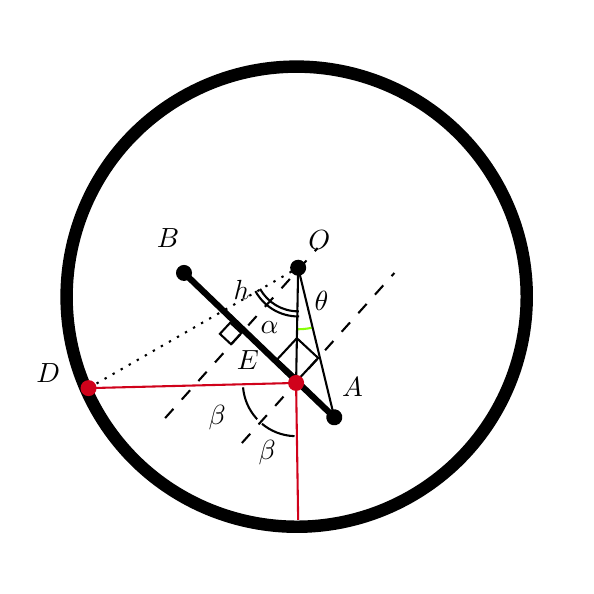
\begin{tikzpicture}[x=0.75pt,y=0.75pt,yscale=-1,xscale=1]
%uncomment if require: \path (0,1136); %set diagram left start at 0, and has height of 1136

%Shape: Arc [id:dp24627552355579385] 
\draw  [draw opacity=0] (192.48,634.42) .. controls (190.11,634.95) and (187.68,635.18) .. (185.27,635.12) -- (186,605.5) -- cycle ; \draw  [color={rgb, 255:red, 135; green, 255; blue, 6 }  ,draw opacity=1 ] (192.48,634.42) .. controls (190.11,634.95) and (187.68,635.18) .. (185.27,635.12) ;  
%Straight Lines [id:da5273070650918834] 
\draw  [dash pattern={on 0.84pt off 2.51pt}]  (85,663.5) -- (186,605.5) ;
%Shape: Ellipse [id:dp9969570961572984] 
\draw  [line width=4.5]  (240.19,715.71) .. controls (187.02,746.04) and (119.33,727.52) .. (89,674.35) .. controls (58.68,621.18) and (77.19,553.49) .. (130.36,523.17) .. controls (183.53,492.84) and (251.22,511.36) .. (281.55,564.53) .. controls (311.88,617.7) and (293.36,685.38) .. (240.19,715.71) -- cycle ;
%Straight Lines [id:da09021004556346202] 
\draw [color={rgb, 255:red, 208; green, 2; blue, 27 }  ,draw opacity=1 ]   (85,663.5) -- (185,661) ;
\draw [shift={(85,663.5)}, rotate = 358.57] [color={rgb, 255:red, 208; green, 2; blue, 27 }  ,draw opacity=1 ][fill={rgb, 255:red, 208; green, 2; blue, 27 }  ,fill opacity=1 ][line width=0.75]      (0, 0) circle [x radius= 3.35, y radius= 3.35]   ;
%Straight Lines [id:da5876905752019481] 
\draw [line width=2.25]    (203.41,677.56) -- (131,608) ;
%Straight Lines [id:da5389790296789774] 
\draw    (185,661) -- (186,605.5) ;
\draw [shift={(186,605.5)}, rotate = 271.03] [color={rgb, 255:red, 0; green, 0; blue, 0 }  ][fill={rgb, 255:red, 0; green, 0; blue, 0 }  ][line width=0.75]      (0, 0) circle [x radius= 3.35, y radius= 3.35]   ;
%Straight Lines [id:da7853938206207205] 
\draw  [dash pattern={on 4.5pt off 4.5pt}]  (158.9,689.93) -- (232.37,608.01) ;
%Shape: Square [id:dp7328130693748438] 
\draw   (175.85,649.71) -- (185.38,639.45) -- (195.64,648.97) -- (186.12,659.23) -- cycle ;

%Shape: Arc [id:dp487213603069387] 
\draw  [draw opacity=0] (186.37,626.5) .. controls (186.25,626.5) and (186.12,626.5) .. (186,626.5) .. controls (178.1,626.5) and (171.22,622.14) .. (167.64,615.7) -- (186,605.5) -- cycle ; \draw   (186.37,626.5) .. controls (186.25,626.5) and (186.12,626.5) .. (186,626.5) .. controls (178.1,626.5) and (171.22,622.14) .. (167.64,615.7) ;  
%Shape: Arc [id:dp43132279819486574] 
\draw  [draw opacity=0] (186.41,628.96) .. controls (186.28,628.96) and (186.14,628.96) .. (186,628.96) .. controls (177.11,628.96) and (169.38,624.02) .. (165.4,616.74) -- (186,605.5) -- cycle ; \draw   (186.41,628.96) .. controls (186.28,628.96) and (186.14,628.96) .. (186,628.96) .. controls (177.11,628.96) and (169.38,624.02) .. (165.4,616.74) ;  
%Straight Lines [id:da9263575201931094] 
\draw    (203.41,677.56) -- (186,605.5) ;
\draw [shift={(203.41,677.56)}, rotate = 256.42] [color={rgb, 255:red, 0; green, 0; blue, 0 }  ][fill={rgb, 255:red, 0; green, 0; blue, 0 }  ][line width=0.75]      (0, 0) circle [x radius= 3.35, y radius= 3.35]   ;
%Shape: Arc [id:dp7470370904695878] 
\draw  [draw opacity=0] (184.24,686.63) .. controls (184.09,686.62) and (183.94,686.62) .. (183.79,686.61) .. controls (177.96,686.33) and (172.69,684.14) .. (168.54,680.66) -- (185,661) -- cycle ; \draw   (184.24,686.63) .. controls (184.09,686.62) and (183.94,686.62) .. (183.79,686.61) .. controls (177.96,686.33) and (172.69,684.14) .. (168.54,680.66) ;  
%Shape: Arc [id:dp5269453343544999] 
\draw  [draw opacity=0] (166.25,678.49) .. controls (166.15,678.38) and (166.05,678.27) .. (165.95,678.16) .. controls (162.05,673.82) and (159.9,668.53) .. (159.45,663.13) -- (185,661) -- cycle ; \draw   (166.25,678.49) .. controls (166.15,678.38) and (166.05,678.27) .. (165.95,678.16) .. controls (162.05,673.82) and (159.9,668.53) .. (159.45,663.13) ;  
%Straight Lines [id:da26928376701497747] 
\draw    (131,608) -- (203.41,677.56) ;
\draw [shift={(131,608)}, rotate = 43.85] [color={rgb, 255:red, 0; green, 0; blue, 0 }  ][fill={rgb, 255:red, 0; green, 0; blue, 0 }  ][line width=0.75]      (0, 0) circle [x radius= 3.35, y radius= 3.35]   ;
%Straight Lines [id:da5929915005421562] 
\draw [color={rgb, 255:red, 208; green, 2; blue, 27 }  ,draw opacity=1 ]   (186,727) -- (185,661) ;
\draw [shift={(185,661)}, rotate = 269.13] [color={rgb, 255:red, 208; green, 2; blue, 27 }  ,draw opacity=1 ][fill={rgb, 255:red, 208; green, 2; blue, 27 }  ,fill opacity=1 ][line width=0.75]      (0, 0) circle [x radius= 3.35, y radius= 3.35]   ;
%Straight Lines [id:da33086310390014084] 
\draw  [dash pattern={on 4.5pt off 4.5pt}]  (121.9,677.93) -- (195.37,596.01) ;
%Shape: Square [id:dp6524763554845552] 
\draw   (148.28,637.36) -- (153.26,631.98) -- (158.64,636.97) -- (153.65,642.34) -- cycle ;

% Text Node
\draw (205.64,656.97) node [anchor=north west][inner sep=0.75pt]   [align=left] {$\displaystyle A$};
% Text Node
\draw (58.41,650.19) node [anchor=north west][inner sep=0.75pt]   [align=left] {$\displaystyle D$};
% Text Node
\draw (189.41,586.19) node [anchor=north west][inner sep=0.75pt]   [align=left] {$\displaystyle O$};
% Text Node
\draw (116.41,585.19) node [anchor=north west][inner sep=0.75pt]   [align=left] {$\displaystyle B$};
% Text Node
\draw (166.4,629.74) node [anchor=north west][inner sep=0.75pt]   [align=left] {$\displaystyle \alpha $};
% Text Node
\draw (192.41,615.19) node [anchor=north west][inner sep=0.75pt]   [align=left] {$\displaystyle \theta $};
% Text Node
\draw (141.41,670.19) node [anchor=north west][inner sep=0.75pt]   [align=left] {$\displaystyle \beta $};
% Text Node
\draw (165.41,687.19) node [anchor=north west][inner sep=0.75pt]   [align=left] {$\displaystyle \beta $};
% Text Node
\draw (155,644) node [anchor=north west][inner sep=0.75pt]   [align=left] {$\displaystyle E$};
% Text Node
\draw (153.41,610.19) node [anchor=north west][inner sep=0.75pt]   [align=left] {$\displaystyle h$};


\end{tikzpicture}


    \end{center}
    Góc $\beta$ được tính bằng
    \begin{align*}
        \beta=60^\circ-\theta 
    \end{align*}
    Ta tính được $h$ bằng:
    \begin{align}
        h=\overline{\text{OA}} \sin(30^\circ)=R\frac{\sin \left( 110^\circ + 60^\circ \right)}{\sin\left( 60^\circ\right)} \sin(30^\circ)=R \frac{\sqrt{3}}{3} \sin \left( 170^\circ \right)
    \end{align}
    Từ đó ta cũng có cạnh $\overline{\text{OE}}$ (xét trong tam giác tạo bởi đường cao $h$ với cạnh $\overline{\text{OE}}$):
    \begin{align}
        \overline{\text{OE}}=\frac{h}{\sin\left(\theta + 30^\circ\right)}
    \end{align}
    Xét $\Delta OED$, từ công thức sine ta có:
    \begin{align*}
        \frac{\overline{\text{OE}}}{\sin \left( 2 \beta - \alpha\right)}=\frac{R}{\sin \left( 2\beta\right)}
    \end{align*}
    Vậy ta tính được $\alpha$ là
    \begin{align}
        \alpha=120^\circ-2\theta - \arcsin \left( \frac{2\sqrt{3}}{3} \sin \left( 170^\circ \right) \cos\left(\theta + 30^\circ \right) \right)
    \end{align}


Như vậy, đồ thị của hệ chính xác là một đường cong nhẹ và tương đối thẳng, nên ta vẫn có thể chấp nhận được đồ thị mà đề bài đã đưa ra.
\\
\end{enumerate}

\textit{Bài toán này được lấy ý tưởng từ bài 1 đề thực hành APhO 2005, với các vật phản xạ bên trong hộp đen không chỉ là lăng trụ mà còn có thể chứa mặt cong lồi lõm nữa: \\
\url{http://asianphysicsolympiad.org/download/past_APhO_roblems/2005_APhO/APhO2005_exp_sol.pdf}
\\
Ngoài bài toán trên, bạn Noid của nhóm ta đã có một chương trình cho một vật kính hình vuông như sau, dành cho các bạn muốn tự thử làm thí nghiệm ảo:
\\
\url{https://editor.p5js.org/ooouuu/full/HeZ6uj_1i}
}